% !TEX encoding = UTF-8 Unicode
\documentclass[10pt]{standalone}\usepackage{tikz,graphicx}
\usepackage{fontspec}
\setmainfont{Arial}
\setsansfont{Arial}\begin{document}

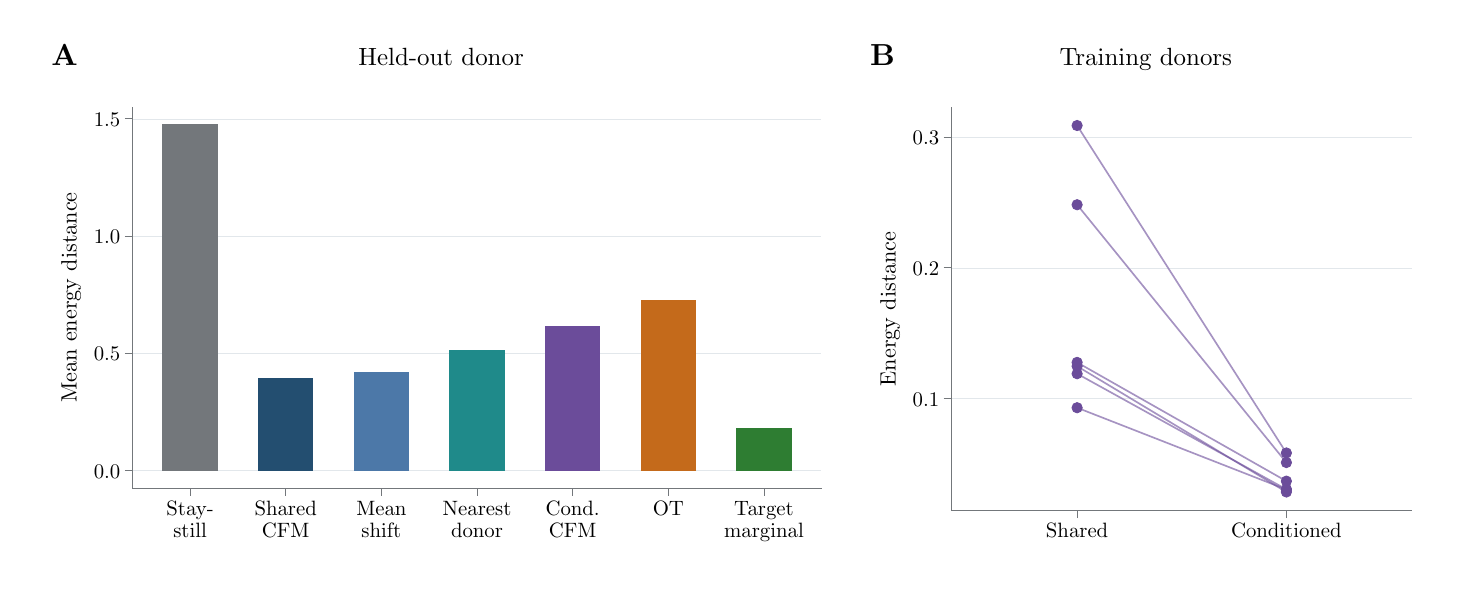
\begin{tikzpicture}[x=1pt,y=1pt]
\definecolor{fillColor}{RGB}{255,255,255}
\path[use as bounding box,fill=fillColor,fill opacity=0.00] (0,0) rectangle (512.15,193.48);
\begin{scope}
\path[clip] (  0.00,  0.00) rectangle (512.15,193.48);
\definecolor{drawColor}{RGB}{0,0,0}

\node[text=drawColor,anchor=base west,inner sep=0pt, outer sep=0pt, scale=  1.10] at (  8.54,179.91) {\bfseries A};

\node[text=drawColor,anchor=base,inner sep=0pt, outer sep=0pt, scale=  0.90] at (149.38,179.92) {Held-out donor};
\end{scope}
\begin{scope}
\path[clip] (  8.54,  4.27) rectangle (290.22,169.86);
\definecolor{fillColor}{RGB}{255,255,255}

\path[fill=fillColor] (  8.54,  4.27) rectangle (290.22,169.86);
\end{scope}
\begin{scope}
\path[clip] ( 37.93, 27.17) rectangle (286.80,164.74);
\definecolor{fillColor}{RGB}{255,255,255}

\path[fill=fillColor] ( 37.93, 27.17) rectangle (286.80,164.74);
\definecolor{drawColor}{RGB}{226,231,235}

\path[draw=drawColor,line width= 0.2pt,line join=round] ( 37.93, 33.43) --
	(286.80, 33.43);

\path[draw=drawColor,line width= 0.2pt,line join=round] ( 37.93, 75.79) --
	(286.80, 75.79);

\path[draw=drawColor,line width= 0.2pt,line join=round] ( 37.93,118.16) --
	(286.80,118.16);

\path[draw=drawColor,line width= 0.2pt,line join=round] ( 37.93,160.52) --
	(286.80,160.52);
\definecolor{fillColor}{RGB}{115,119,123}

\path[fill=fillColor] ( 48.65, 33.43) rectangle ( 68.69,158.49);
\definecolor{fillColor}{RGB}{35,78,112}

\path[fill=fillColor] ( 83.21, 33.43) rectangle (103.26, 66.87);
\definecolor{fillColor}{RGB}{76,120,168}

\path[fill=fillColor] (117.78, 33.43) rectangle (137.83, 68.89);
\definecolor{fillColor}{RGB}{31,138,138}

\path[fill=fillColor] (152.34, 33.43) rectangle (172.39, 77.04);
\definecolor{fillColor}{RGB}{107,76,154}

\path[fill=fillColor] (186.91, 33.43) rectangle (206.96, 85.76);
\definecolor{fillColor}{RGB}{196,106,27}

\path[fill=fillColor] (221.47, 33.43) rectangle (241.52, 95.14);
\definecolor{fillColor}{RGB}{46,125,50}

\path[fill=fillColor] (256.04, 33.43) rectangle (276.09, 48.83);
\end{scope}
\begin{scope}
\path[clip] (  0.00,  0.00) rectangle (512.15,193.48);
\definecolor{drawColor}{RGB}{115,119,123}

\path[draw=drawColor,line width= 0.3pt,line join=round,line cap=rect] ( 37.93, 27.17) --
	( 37.93,164.74);
\end{scope}
\begin{scope}
\path[clip] (  0.00,  0.00) rectangle (512.15,193.48);
\definecolor{drawColor}{RGB}{0,0,0}

\node[text=drawColor,anchor=base east,inner sep=0pt, outer sep=0pt, scale=  0.75] at ( 33.49, 30.74) {0.0};

\node[text=drawColor,anchor=base east,inner sep=0pt, outer sep=0pt, scale=  0.75] at ( 33.49, 73.11) {0.5};

\node[text=drawColor,anchor=base east,inner sep=0pt, outer sep=0pt, scale=  0.75] at ( 33.49,115.47) {1.0};

\node[text=drawColor,anchor=base east,inner sep=0pt, outer sep=0pt, scale=  0.75] at ( 33.49,157.84) {1.5};
\end{scope}
\begin{scope}
\path[clip] (  0.00,  0.00) rectangle (512.15,193.48);
\definecolor{drawColor}{RGB}{115,119,123}

\path[draw=drawColor,line width= 0.3pt,line join=round] ( 35.09, 33.43) --
	( 37.93, 33.43);

\path[draw=drawColor,line width= 0.3pt,line join=round] ( 35.09, 75.79) --
	( 37.93, 75.79);

\path[draw=drawColor,line width= 0.3pt,line join=round] ( 35.09,118.16) --
	( 37.93,118.16);

\path[draw=drawColor,line width= 0.3pt,line join=round] ( 35.09,160.52) --
	( 37.93,160.52);
\end{scope}
\begin{scope}
\path[clip] (  0.00,  0.00) rectangle (512.15,193.48);
\definecolor{drawColor}{RGB}{115,119,123}

\path[draw=drawColor,line width= 0.3pt,line join=round,line cap=rect] ( 37.93, 27.17) --
	(286.80, 27.17);
\end{scope}
\begin{scope}
\path[clip] (  0.00,  0.00) rectangle (512.15,193.48);
\definecolor{drawColor}{RGB}{115,119,123}

\path[draw=drawColor,line width= 0.3pt,line join=round] ( 58.67, 24.33) --
	( 58.67, 27.17);

\path[draw=drawColor,line width= 0.3pt,line join=round] ( 93.24, 24.33) --
	( 93.24, 27.17);

\path[draw=drawColor,line width= 0.3pt,line join=round] (127.80, 24.33) --
	(127.80, 27.17);

\path[draw=drawColor,line width= 0.3pt,line join=round] (162.37, 24.33) --
	(162.37, 27.17);

\path[draw=drawColor,line width= 0.3pt,line join=round] (196.93, 24.33) --
	(196.93, 27.17);

\path[draw=drawColor,line width= 0.3pt,line join=round] (231.50, 24.33) --
	(231.50, 27.17);

\path[draw=drawColor,line width= 0.3pt,line join=round] (266.06, 24.33) --
	(266.06, 27.17);
\end{scope}
\begin{scope}
\path[clip] (  0.00,  0.00) rectangle (512.15,193.48);
\definecolor{drawColor}{RGB}{0,0,0}

\node[text=drawColor,anchor=base,inner sep=0pt, outer sep=0pt, scale=  0.75] at ( 58.67, 17.36) {Stay-};

\node[text=drawColor,anchor=base,inner sep=0pt, outer sep=0pt, scale=  0.75] at ( 58.67,  9.26) {still};

\node[text=drawColor,anchor=base,inner sep=0pt, outer sep=0pt, scale=  0.75] at ( 93.24, 17.36) {Shared};

\node[text=drawColor,anchor=base,inner sep=0pt, outer sep=0pt, scale=  0.75] at ( 93.24,  9.26) {CFM};

\node[text=drawColor,anchor=base,inner sep=0pt, outer sep=0pt, scale=  0.75] at (127.80, 17.36) {Mean};

\node[text=drawColor,anchor=base,inner sep=0pt, outer sep=0pt, scale=  0.75] at (127.80,  9.26) {shift};

\node[text=drawColor,anchor=base,inner sep=0pt, outer sep=0pt, scale=  0.75] at (162.37, 17.36) {Nearest};

\node[text=drawColor,anchor=base,inner sep=0pt, outer sep=0pt, scale=  0.75] at (162.37,  9.26) {donor};

\node[text=drawColor,anchor=base,inner sep=0pt, outer sep=0pt, scale=  0.75] at (196.93, 17.36) {Cond.};

\node[text=drawColor,anchor=base,inner sep=0pt, outer sep=0pt, scale=  0.75] at (196.93,  9.26) {CFM};

\node[text=drawColor,anchor=base,inner sep=0pt, outer sep=0pt, scale=  0.75] at (231.50, 17.36) {OT};

\node[text=drawColor,anchor=base,inner sep=0pt, outer sep=0pt, scale=  0.75] at (266.06, 17.36) {Target};

\node[text=drawColor,anchor=base,inner sep=0pt, outer sep=0pt, scale=  0.75] at (266.06,  9.26) {marginal};
\end{scope}
\begin{scope}
\path[clip] (  0.00,  0.00) rectangle (512.15,193.48);
\definecolor{drawColor}{RGB}{0,0,0}

\node[text=drawColor,rotate= 90.00,anchor=base,inner sep=0pt, outer sep=0pt, scale=  0.80] at ( 17.68, 95.96) {Mean energy distance};
\end{scope}
\begin{scope}
\path[clip] (  0.00,  0.00) rectangle (512.15,193.48);
\definecolor{drawColor}{RGB}{0,0,0}

\node[text=drawColor,anchor=base west,inner sep=0pt, outer sep=0pt, scale=  1.10] at (304.44,179.91) {\bfseries B};

\node[text=drawColor,anchor=base,inner sep=0pt, outer sep=0pt, scale=  0.90] at (404.03,179.92) {Training donors};
\end{scope}
\begin{scope}
\path[clip] (304.44,  4.27) rectangle (503.61,169.86);
\definecolor{fillColor}{RGB}{255,255,255}

\path[fill=fillColor] (304.44,  4.27) rectangle (503.61,169.86);
\end{scope}
\begin{scope}
\path[clip] (333.84, 19.07) rectangle (500.20,164.74);
\definecolor{fillColor}{RGB}{255,255,255}

\path[fill=fillColor] (333.84, 19.07) rectangle (500.20,164.74);
\definecolor{drawColor}{RGB}{226,231,235}

\path[draw=drawColor,line width= 0.2pt,line join=round] (333.84, 59.44) --
	(500.20, 59.44);

\path[draw=drawColor,line width= 0.2pt,line join=round] (333.84,106.69) --
	(500.20,106.69);

\path[draw=drawColor,line width= 0.2pt,line join=round] (333.84,153.93) --
	(500.20,153.93);
\definecolor{drawColor}{RGB}{107,76,154}

\path[draw=drawColor,draw opacity=0.60,line width= 0.6pt,line join=round] (379.21, 72.53) --
	(454.83, 29.62);

\path[draw=drawColor,draw opacity=0.60,line width= 0.6pt,line join=round] (379.21, 56.15) --
	(454.83, 26.59);

\path[draw=drawColor,draw opacity=0.60,line width= 0.6pt,line join=round] (379.21,129.50) --
	(454.83, 36.34);

\path[draw=drawColor,draw opacity=0.60,line width= 0.6pt,line join=round] (379.21, 71.16) --
	(454.83, 25.70);

\path[draw=drawColor,draw opacity=0.60,line width= 0.6pt,line join=round] (379.21,158.12) --
	(454.83, 39.80);

\path[draw=drawColor,draw opacity=0.60,line width= 0.6pt,line join=round] (379.21, 68.44) --
	(454.83, 26.64);
\definecolor{drawColor}{RGB}{107,76,154}
\definecolor{fillColor}{RGB}{107,76,154}

\path[draw=drawColor,line width= 0.3pt,line join=round,line cap=round,fill=fillColor] (379.21, 72.53) circle (  1.87);

\path[draw=drawColor,line width= 0.3pt,line join=round,line cap=round,fill=fillColor] (454.83, 29.62) circle (  1.87);

\path[draw=drawColor,line width= 0.3pt,line join=round,line cap=round,fill=fillColor] (379.21, 56.15) circle (  1.87);

\path[draw=drawColor,line width= 0.3pt,line join=round,line cap=round,fill=fillColor] (454.83, 26.59) circle (  1.87);

\path[draw=drawColor,line width= 0.3pt,line join=round,line cap=round,fill=fillColor] (379.21,129.50) circle (  1.87);

\path[draw=drawColor,line width= 0.3pt,line join=round,line cap=round,fill=fillColor] (454.83, 36.34) circle (  1.87);

\path[draw=drawColor,line width= 0.3pt,line join=round,line cap=round,fill=fillColor] (379.21, 71.16) circle (  1.87);

\path[draw=drawColor,line width= 0.3pt,line join=round,line cap=round,fill=fillColor] (454.83, 25.70) circle (  1.87);

\path[draw=drawColor,line width= 0.3pt,line join=round,line cap=round,fill=fillColor] (379.21,158.12) circle (  1.87);

\path[draw=drawColor,line width= 0.3pt,line join=round,line cap=round,fill=fillColor] (454.83, 39.80) circle (  1.87);

\path[draw=drawColor,line width= 0.3pt,line join=round,line cap=round,fill=fillColor] (379.21, 68.44) circle (  1.87);

\path[draw=drawColor,line width= 0.3pt,line join=round,line cap=round,fill=fillColor] (454.83, 26.64) circle (  1.87);
\end{scope}
\begin{scope}
\path[clip] (  0.00,  0.00) rectangle (512.15,193.48);
\definecolor{drawColor}{RGB}{115,119,123}

\path[draw=drawColor,line width= 0.3pt,line join=round,line cap=rect] (333.84, 19.07) --
	(333.84,164.74);
\end{scope}
\begin{scope}
\path[clip] (  0.00,  0.00) rectangle (512.15,193.48);
\definecolor{drawColor}{RGB}{0,0,0}

\node[text=drawColor,anchor=base east,inner sep=0pt, outer sep=0pt, scale=  0.75] at (329.39, 56.76) {0.1};

\node[text=drawColor,anchor=base east,inner sep=0pt, outer sep=0pt, scale=  0.75] at (329.39,104.00) {0.2};

\node[text=drawColor,anchor=base east,inner sep=0pt, outer sep=0pt, scale=  0.75] at (329.39,151.25) {0.3};
\end{scope}
\begin{scope}
\path[clip] (  0.00,  0.00) rectangle (512.15,193.48);
\definecolor{drawColor}{RGB}{115,119,123}

\path[draw=drawColor,line width= 0.3pt,line join=round] (330.99, 59.44) --
	(333.84, 59.44);

\path[draw=drawColor,line width= 0.3pt,line join=round] (330.99,106.69) --
	(333.84,106.69);

\path[draw=drawColor,line width= 0.3pt,line join=round] (330.99,153.93) --
	(333.84,153.93);
\end{scope}
\begin{scope}
\path[clip] (  0.00,  0.00) rectangle (512.15,193.48);
\definecolor{drawColor}{RGB}{115,119,123}

\path[draw=drawColor,line width= 0.3pt,line join=round,line cap=rect] (333.84, 19.07) --
	(500.20, 19.07);
\end{scope}
\begin{scope}
\path[clip] (  0.00,  0.00) rectangle (512.15,193.48);
\definecolor{drawColor}{RGB}{115,119,123}

\path[draw=drawColor,line width= 0.3pt,line join=round] (379.21, 16.23) --
	(379.21, 19.07);

\path[draw=drawColor,line width= 0.3pt,line join=round] (454.83, 16.23) --
	(454.83, 19.07);
\end{scope}
\begin{scope}
\path[clip] (  0.00,  0.00) rectangle (512.15,193.48);
\definecolor{drawColor}{RGB}{0,0,0}

\node[text=drawColor,anchor=base,inner sep=0pt, outer sep=0pt, scale=  0.75] at (379.21,  9.26) {Shared};

\node[text=drawColor,anchor=base,inner sep=0pt, outer sep=0pt, scale=  0.75] at (454.83,  9.26) {Conditioned};
\end{scope}
\begin{scope}
\path[clip] (  0.00,  0.00) rectangle (512.15,193.48);
\definecolor{drawColor}{RGB}{0,0,0}

\node[text=drawColor,rotate= 90.00,anchor=base,inner sep=0pt, outer sep=0pt, scale=  0.80] at (313.59, 91.91) {Energy distance};
\end{scope}
\end{tikzpicture}

\end{document}
